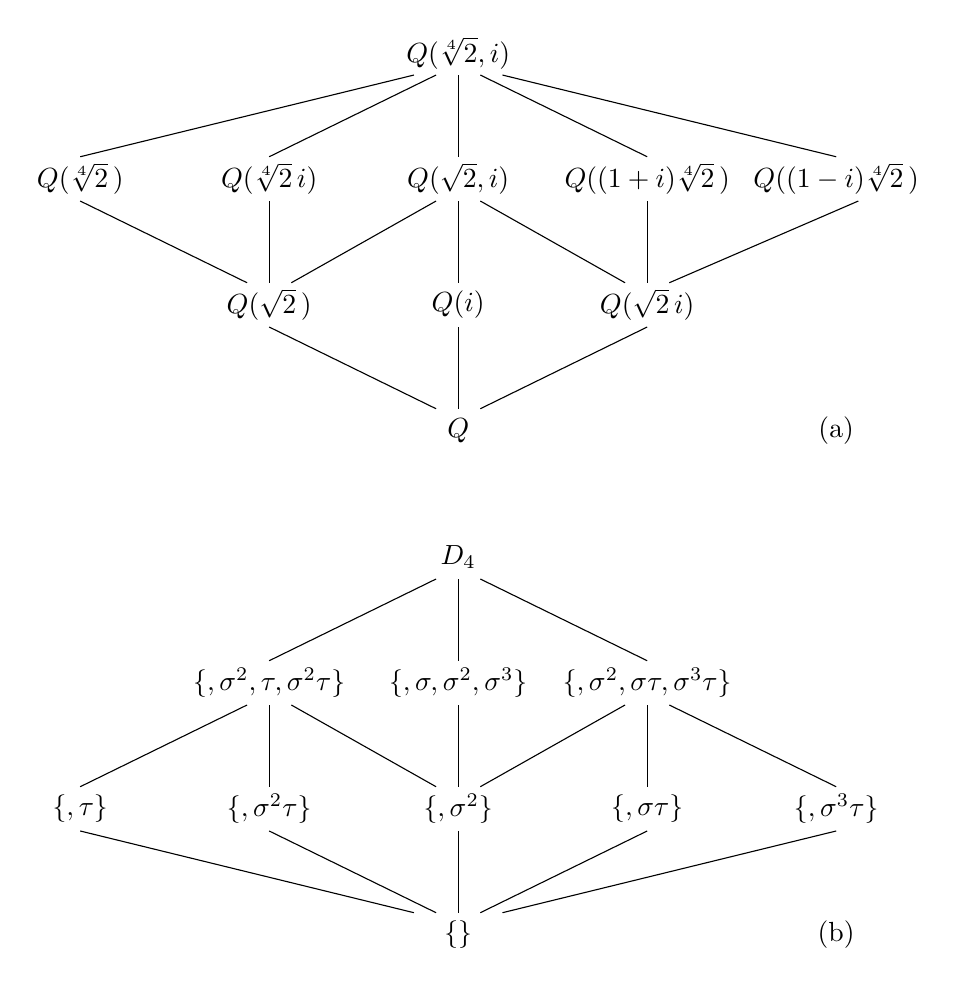
\begin{tikzpicture}[scale=0.8]

%Subfields of  Q-4-root-2-comma-i

\coordinate (Q-4-root-2-comma-i) at (0,14);

\coordinate (Q-4-root-2) at (-6,12);
\coordinate (Q-4-root-2-i) at (-3,12);
\coordinate (Q-2-comma-i) at (0,12);
\coordinate (Q-1-plus-i-4-root-2) at (3,12);
\coordinate (Q-1-minus-i-4-root-2) at (6,12);

\coordinate (Q-2-i) at (3,10);
\coordinate (Q-i) at (0,10);
\coordinate (Q-2) at (-3,10);

\coordinate (Q) at (0,8);
\coordinate (label-a) at (6,8);

\node at (Q-4-root-2-comma-i)  {${\mathbb Q}(\sqrt[4]{2}, i )$};

\node at (Q-4-root-2)  {${\mathbb Q}( \sqrt[4]{2}\, )$};
\node at (Q-4-root-2-i)  {${\mathbb Q}( \sqrt[4]{2}\, i)$};
\node at (Q-2-comma-i)  {${\mathbb Q}( \sqrt{2}, i)$};
\node at (Q-1-plus-i-4-root-2)  {${\mathbb Q}((1 + i) \sqrt[4]{2}\,)$};
\node at (Q-1-minus-i-4-root-2)  {${\mathbb Q}( (1 - i)\sqrt[4]{2}\, )$};

\node at (Q-2)  {${\mathbb Q}(\sqrt{2}\, )$};
\node at (Q-i)  {${\mathbb Q}(i)$};
\node at (Q-2-i)  {${\mathbb Q}(\sqrt{2}\, i)$};

\node at (Q)  {${\mathbb Q}$};
\node at (label-a) {(a)};


\draw  ([xshift=-20,yshift=-10]Q-4-root-2-comma-i) -- ([yshift=10]Q-4-root-2);
\draw  ([xshift=-10,yshift=-10]Q-4-root-2-comma-i) -- ([yshift=10]Q-4-root-2-i);
\draw  ([yshift=-10]Q-4-root-2-comma-i) -- ([yshift=10]Q-2-comma-i);
\draw  ([xshift=10,yshift=-10]Q-4-root-2-comma-i) -- ([yshift=10]Q-1-plus-i-4-root-2);
\draw  ([xshift=20,yshift=-10]Q-4-root-2-comma-i) -- ([yshift=10]Q-1-minus-i-4-root-2) ;

\draw  ([yshift=-10]Q-4-root-2) -- ([xshift=-10,yshift=10]Q-2);
\draw  ([yshift=-10]Q-4-root-2-i) -- ([yshift=10]Q-2);
\draw  ([xshift=-10,yshift=-10]Q-2-comma-i) --([xshift=10,yshift=10]Q-2);
\draw   ([yshift=-10]Q-2-comma-i) -- ([yshift=10]Q-i);

\draw  ([xshift=10,yshift=-10]Q-2-comma-i) -- ([xshift=-10,yshift=10]Q-2-i);
\draw  ([yshift=-10]Q-1-plus-i-4-root-2) -- ([yshift=10]Q-2-i);
\draw  ([xshift=10,yshift=-10]Q-1-minus-i-4-root-2) -- ([xshift=10,yshift=10]Q-2-i);


\draw  ([yshift=-10]Q-2) -- ([xshift=-10,yshift=10]Q);
\draw  ([yshift=-10]Q-i) -- ([yshift=10]Q);
\draw  ([yshift=-10]Q-2-i) -- ([xshift=10,yshift=10]Q);

%Galois Group of D4

\coordinate (D4) at (0,6);

\coordinate (id-sigma-2-tau-sigma-2-tau) at (-3,4);
\coordinate (id-sigma-2-sigma-2-sigma-3) at (0,4);
\coordinate (id-sigma-2-sigma-tau-sigma-3-tau) at (3,4);

\coordinate (id-tau) at (-6,2);
\coordinate (id-sigma-2-tau) at (-3,2);
\coordinate (id-sigma-2) at (0,2);
\coordinate (id-sigma-tau) at (3,2);
\coordinate (id-sigma-3-tau) at (6,2);

\coordinate (id) at (0,0);
\coordinate (label-b) at (6,0);

\node at (D4)  {$D_4$};

\node at (id-sigma-2-tau-sigma-2-tau)  {$\{  \identity, \sigma^2, \tau, \sigma^2 \tau \}$};
\node at (id-sigma-2-sigma-2-sigma-3)  {$\{  \identity, \sigma, \sigma^2, \sigma^3 \}$};
\node at (id-sigma-2-sigma-tau-sigma-3-tau)  {$\{  \identity, \sigma^2, \sigma \tau, \sigma^3 \tau \}$};

\node at (id-tau)  {$\{  \identity, \tau \}$};
\node at (id-sigma-2-tau)  {$\{  \identity, \sigma^2 \tau \}$};
\node at (id-sigma-2)  {$\{  \identity, \sigma^2 \}$};
\node at (id-sigma-tau)  {$\{  \identity, \sigma \tau \}$};
\node at (id-sigma-3-tau)  {$\{  \identity, \sigma^3 \tau \}$};

\node at (id)  {$\{  \identity \}$};
\node at (label-b) {(b)};

\draw  ([xshift=-10,yshift=-10]D4) -- ([yshift=10]id-sigma-2-tau-sigma-2-tau);
\draw  ([yshift=-10]D4) -- ([yshift=10]id-sigma-2-sigma-2-sigma-3);
\draw  ([xshift=10,yshift=-10]D4) -- ([yshift=10]id-sigma-2-sigma-tau-sigma-3-tau);

\draw ([xshift=-10,yshift=-10]id-sigma-2-tau-sigma-2-tau) -- ([yshift=10]id-tau);
\draw ([yshift=-10]id-sigma-2-tau-sigma-2-tau) -- ([yshift=10]id-sigma-2-tau);
\draw  ([xshift=10,yshift=-10]id-sigma-2-tau-sigma-2-tau) -- ([xshift=-10,yshift=10]id-sigma-2);
\draw   ([yshift=-10]id-sigma-2-sigma-2-sigma-3) -- ([yshift=10]id-sigma-2);
\draw  ([xshift=-10,yshift=-10]id-sigma-2-sigma-tau-sigma-3-tau) -- ([xshift=10,yshift=10]id-sigma-2);
\draw  ([yshift=-10]id-sigma-2-sigma-tau-sigma-3-tau) -- ([yshift=10]id-sigma-tau);
\draw  ([xshift=10,yshift=-10]id-sigma-2-sigma-tau-sigma-3-tau) -- ([yshift=10]id-sigma-3-tau);


\draw  ([yshift=-10]id-tau) -- ([xshift=-20,yshift=10]id);
\draw  ([yshift=-10]id-sigma-2-tau) -- ([xshift=-10,yshift=10]id);
\draw  ([yshift=-10]id-sigma-2) -- ([yshift=10]id);
\draw  ([yshift=-10]id-sigma-tau) -- ([xshift=10,yshift=10]id);
\draw  ([yshift=-10]id-sigma-3-tau) -- ([xshift=20,yshift=10]id);

\end{tikzpicture}
